\subsection{General Process and Application Setup}
\label{sub:process}
The crucial role in the process of enabling clinicians to analyse their clinical data is played by the statistician: registered or approved by an administrator they are allowed to perform significant changes to the \gls{SKB} which is required to provide the clinicians with a sophisticated foundation for their analyses. 

\begin{figure}[htbp]
\centering
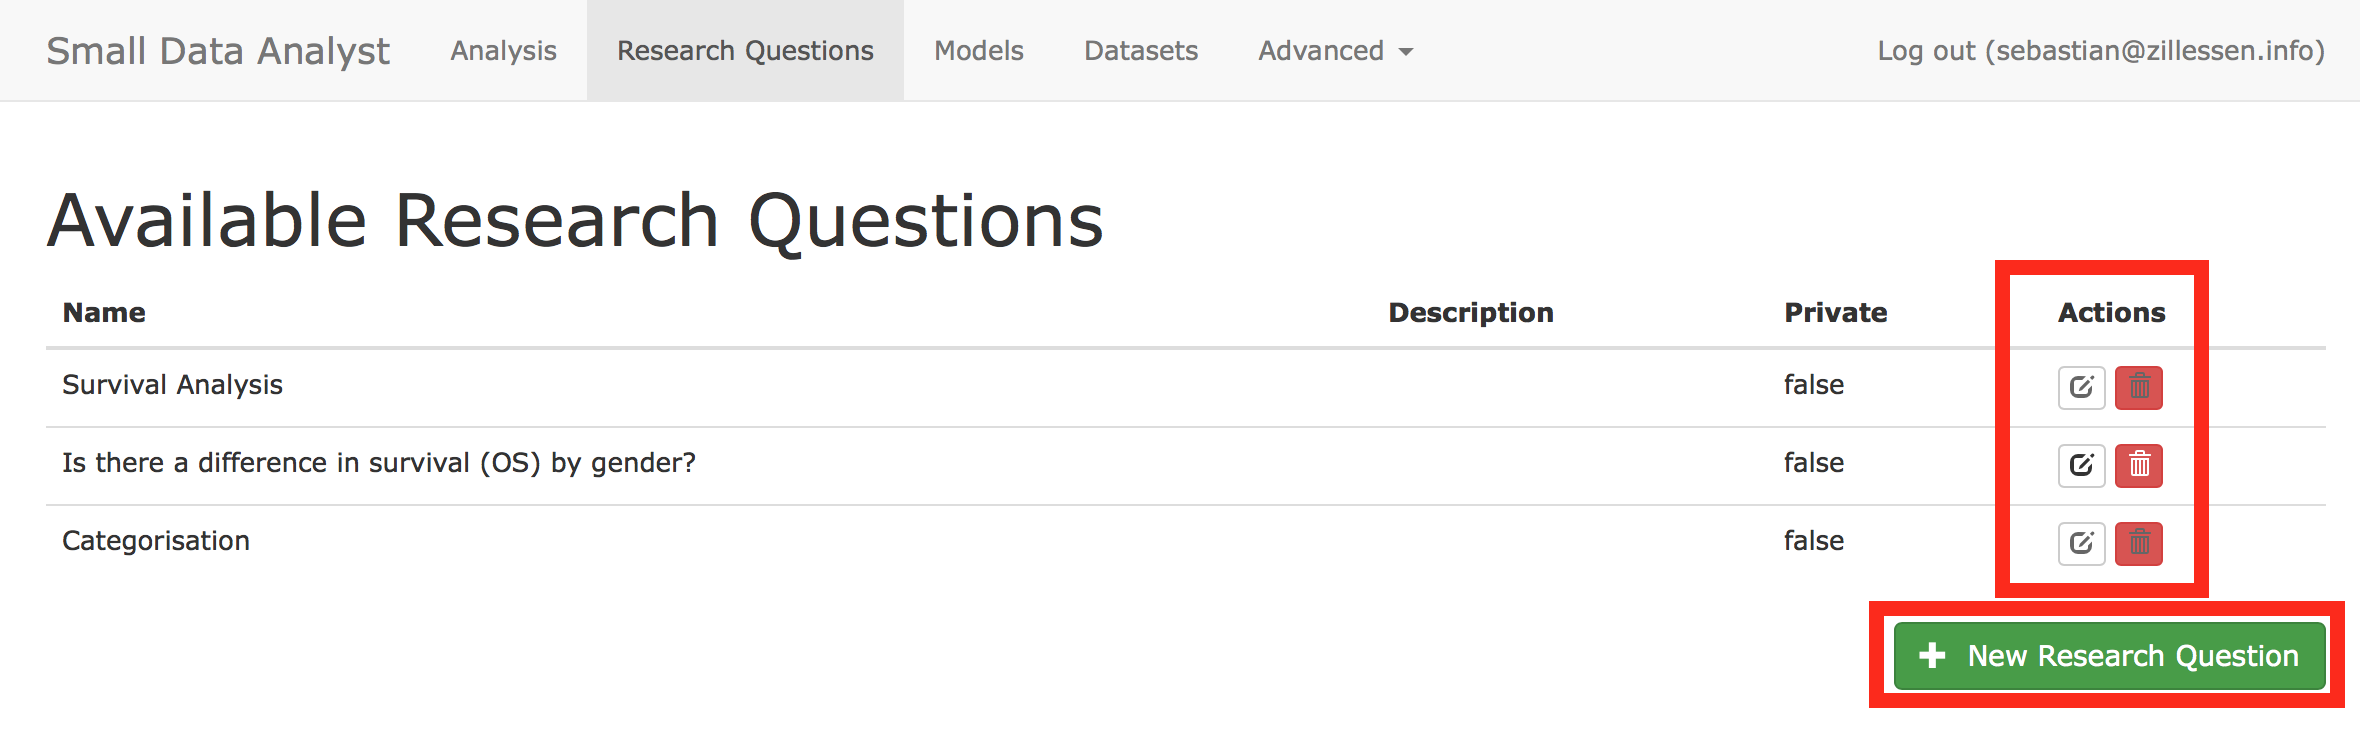
\includegraphics[width=0.8\textwidth]{figures/ui_RQ}
\caption{Listing of research questions: The highlighted areas might not be available, depending on the access rights of the currently logged-in user.}
\label{fig:ui:rq}
\end{figure}

To do so a \textbf{statistician} will first prepare the system involving the following steps:

\begin{enumerate}
	\item Defining a research question (see \autoref{fig:ui:rq}).
	\item Assigning suitable models (see \autoref{fig:ui:model}) to a research question.
	\item Providing assumptions (see \autoref{fig:ui:assumption}) that need to hold to make this model a possible model in a particular analysis.
	\item Defining (global) preferences to express a particular order between models in certain contexts that apply if a certain assumption holds (see \autoref{fig:ui:preference}).
\end{enumerate}

\bigskip

A \textbf{clinician} can then initialise a new analysis by performing the following steps:
 
\begin{enumerate}
	\item Uploading a data set that has been acquired during a clinical study.
	\item Optionally expressing (private) preferences between different models.
	\item Generating a new analysis related to a research question and providing the answers required by the system to generate a list of possible models.
	\item Answering further questions that might arise during the evaluation of the possible models to apply context domain specific preferences on the data set.
\end{enumerate}
\bigskip

By applying this workflow, \textbf{clinicians} will be able to make data-driven decisions that are based on the expertise entered by a \textbf{statistician}.
